%!TEX root = ../thesis.tex

\chapter{Analyse} % (fold)
\label{cha:analyse}

%\todo[inline]{Inhalt: wass gibt es, was muss neu gemacht werden}
%\todo[inline]{Aufteilen in Szenarien: Datenaustausch, Übertragung...}

Bevor nun ein System entwickelt werden kann, das die Synchronisation von Diskussionen auf Lernplattformen und sozialen Online-Netzwerken ermöglicht, muss erst eine Analyse der nötigen Komponenten durchgeführt werden. Es muss überprüft werden welche davon neu entwickelt und welche schon vorhanden sind. Diese Analyse soll anhand eines Beispielszenarios geschehen, dass die Schritte zeigt wie ein Beitrag von einer Webseite A in eine zweite Webseite B synchronisiert werden kann. 

\section{Ein Beispielszenario für die Synchronisation von Beiträgen} % (fold)
\label{sec:analyse_beispiel}

% section neuen_beitrag_verfassen (end)
Der Anfang wird damit gemacht, dass ein Beitrag zum Synchronisieren vorhanden sein muss (Diese Schritte sind nicht Teil des fertigen Systems). Zum Beispiel geht ein Student in das Forum seiner Veranstaltung auf der Webseite A und in den Thread zur aktuellen Übung, weil er zu ihr eine Frage hat. Er schreibt also einen neuen Beitrag in das Eingabefeld und schickt es ab. Dieser wird dann an die Webseite A geschickt, im dortigen Format (Format A) in eine Datenbank oder Ähnliches geschrieben und als neuer Beitrag im Thread angezeigt (siehe Abbildung \ref{fig:beutzer_erstellt_beitrag_a}). Da eine andere Webseite B das Format von Webseite A in der Regel nicht versteht, muss in einen nächsten Schritt der Beitrag aus der Datenbank gelesen und auf irgendeine Art konvertiert werden. 

\begin{figure}[ht]
     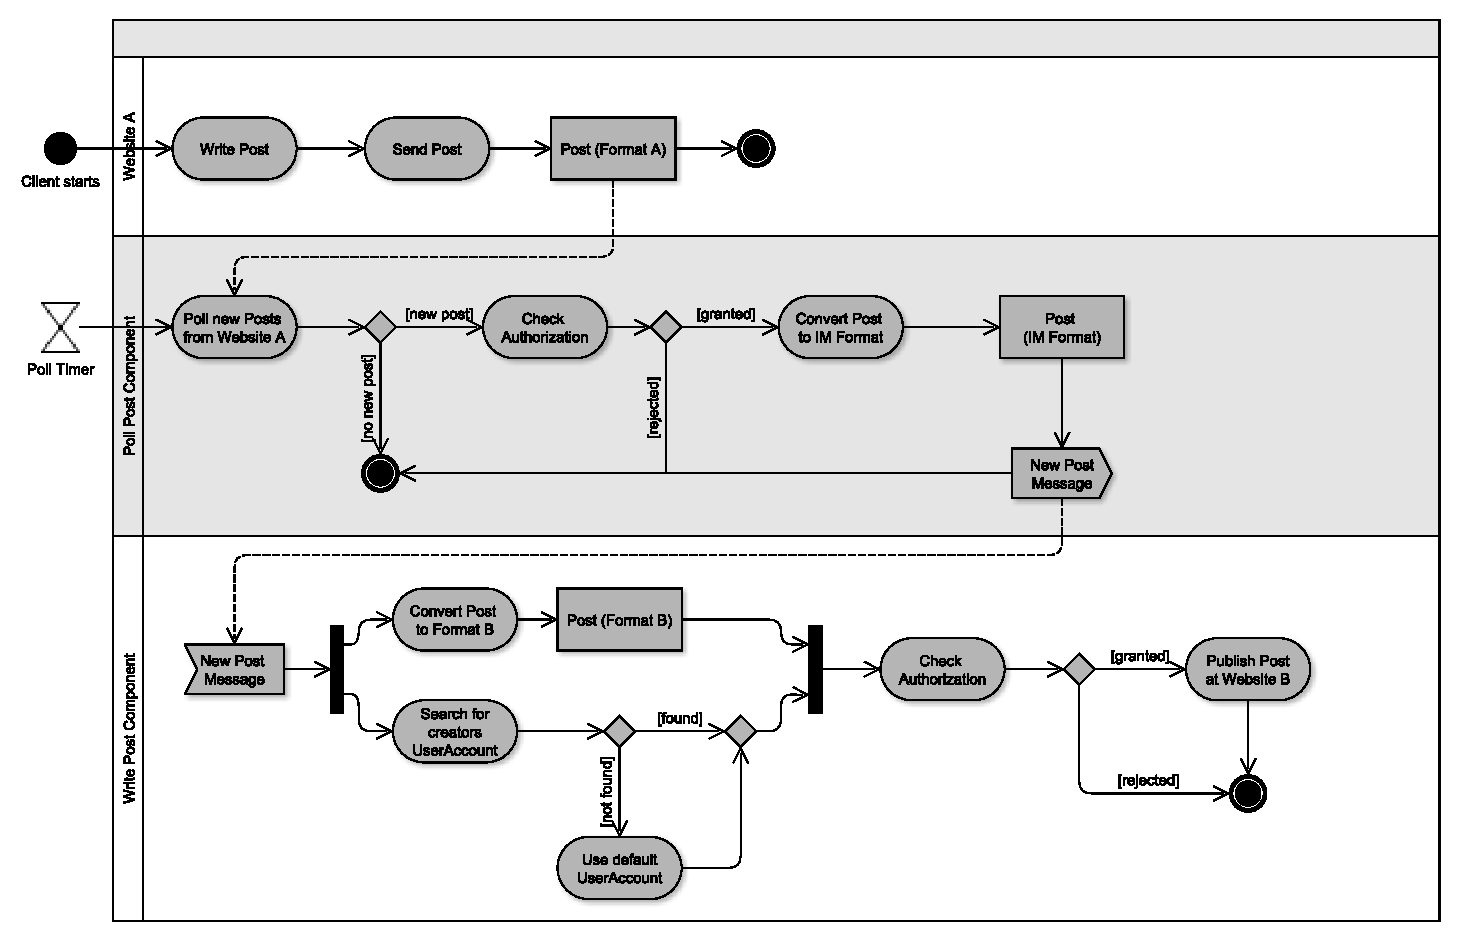
\includegraphics[
        width=\textwidth,
        keepaspectratio=true,
        clip=true,
        trim= 0 338 0 27
    ]{assets/images/activitydiagram_post_as_user_check_authorization.pdf}
    \caption{Benutzer erstellt einen Beitrag auf der Webseite A.}
    \label{fig:beutzer_erstellt_beitrag_a}
\end{figure}

\subsection{Datenkonvertierung} % (fold)
\label{sub:datenkonvertierung}

Abbildung \ref{fig:lesen_von_beitrag_und_convertieren} zeigt den Ablauf, wie Beiträge von der Webseite A gelesen und konvertiert werden. Dazu müssen zuerst die Daten über eine öffentliche API vom Server der Webseite A heruntergeladen werden. Da im Allgemeinen nicht automatisch bekannt ist, wann ein neuer Beitrag vorhanden ist, müssen der Server in zeitlichen Abständen abgefragt (\emph{Polling} genannt) und die zurückgelieferten Daten nach neuen Beiträgen durchsucht werden. Sind neue Beiträge gefunden worden, können diese nicht direkt an die Webseite B geschickt werden, da sich diese in der Regel im verwendeten Datenformat unterscheiden. Diese müssen zuvor untereinander konvertiert werden.

Die einfachste Möglichkeit wäre die Daten von Webseite A, die in Format A vorliegen, in das Format B von Webseite B zu konvertieren. Bei zwei Formaten ist dies noch sehr einfach. Es müsste lediglich ein Konverter von Format A nach Format B und einer in die umgekehrte Richtung implementiert werden. Für den Fall, dass ein weiteres Webseite C unterstützt werden soll, würde ich die Anzahl an notwendigen Konvertern , wie Tabelle \ref{tbl:anzahl_konvertern_bei_drei_netzwerken} zeigt, auf Sechs erhöhen.

\begin{table}[ht]
    \centering
    \caption{Anzahl Konverter bei drei Webseiten}
    
    \begin{tabular}{c|c|c|c|c}
        % Zeile 1
        \multicolumn{2}{c|}{\multirow{2}{*}{}} & 
        \multicolumn{3}{|c}{\textbf{Nach}}   \\ 
        \cline{3-5} 

        % Zeile 2
        \multicolumn{2}{c|}{} & 
        \textbf{Webseite A} & 
        \textbf{Webseite B} & 
        \textbf{Webseite C} \\ 
        \hline

        % Zeile 3
        \multirow{3}{*}{Von} & 
        \textbf{Webseite A} & 
        -&            
        $ \times $ &            
        $ \times $ \\ 
        \cline{2-5} 

        % Zeile 4
        & 
        \textbf{Webseite B} &            
        $ \times $ &            
        -&            
        $ \times $ \\ 
        \cline{2-5} 
         
        % Zeile 5
        & 
        \textbf{Webseite C} &            
        $ \times $ &            
        $ \times $ &            
        -\\
    \end{tabular}
    \label{tbl:anzahl_konvertern_bei_drei_netzwerken}
\end{table}

Nimmt man an $n_{ws}$ sei eine beliebige Anzahl sozialer Netzwerke, entspricht die Anzahl der notwendiger Konverter $ n_{k1} = n_{ws}*(n_{ws}-1) $, da für jedes Netzwerk ein Konverter in alle anderen Netzwerke erzeugt werden muss. Sollen nur Zwei oder Drei Netzwerke unterstützt werden ist der Aufwand noch sehr überschaubar, bei mehr kann dies aber sehr Aufwendig werden. 

\begin{figure}[ht]
    \centering
    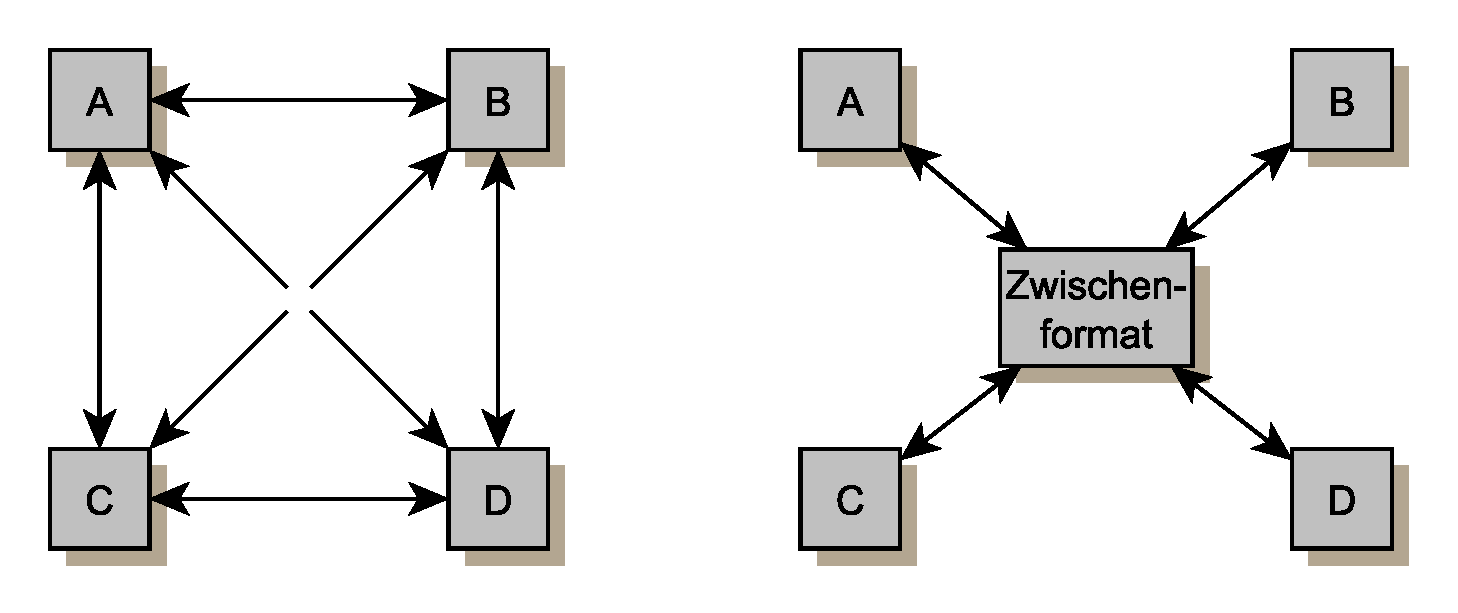
\includegraphics[
        width=0.7\textwidth,
        keepaspectratio=true
    ]{assets/images/interlingua_vs_allvsall}
    \caption{Komplexität ohne und mit dem Einsatz eines Zwischenformats - Originalbild: \cite{Uschold1996a}}
    \label{fig:interlingua_vs_all}
\end{figure}

Eine elegantere Methode für die Lösung dieses Problems, welche die Anzahl zu implementierender Konverter in Grenzen halten kann, wäre die Einführung eines Zwischenformates (auch Inter-Lingua, in Abbildung \ref{fig:lesen_von_beitrag_und_convertieren} als \enquote{IM Format} bezeichnet) \cite[S.\,9]{Uschold1996a}. Geht man davon aus, dass die Daten aller Webseiten nur in dieses Zwischenformat geschrieben und aus diesem gelesen werden müssen, würde sich der Aufwand auf maximal zwei Konverter je Webseite reduzieren. Für eine beliebige Anzahl Webseiten wären also $ n_{k2} = n_{ws} * 2 $ Konverter nötig. Nachteile hätte dieser Ansatz nur für $ n_{ws} = 2 $ und $ n_{ws}=3$ , da in diesen Fällen mehr beziehungsweise gleich viele Konverter gegenüber der ersten Methode erforderlich wären. Erhöht man die Anzahl Webseiten jedoch nur geringfügig, sinkt die Menge an Konvertern sichtbar. Für $ n_{ws} = 4 $ wären es $ n_{k2} = 8 $ statt $ n_{k1} = 12 $ (siehe Abbildung \ref{fig:interlingua_vs_all}) und für $ n_{ws} = 5 $ ergibt sich $ n_{k2} = 10 $ statt $ n_{k1} = 20 $ Konvertern. Gleichzeitig können so syntaktische Unterschiede in den einzelnen Formaten angeglichen werden, was sie leichter handhabbar macht. 

\begin{figure}[ht]
    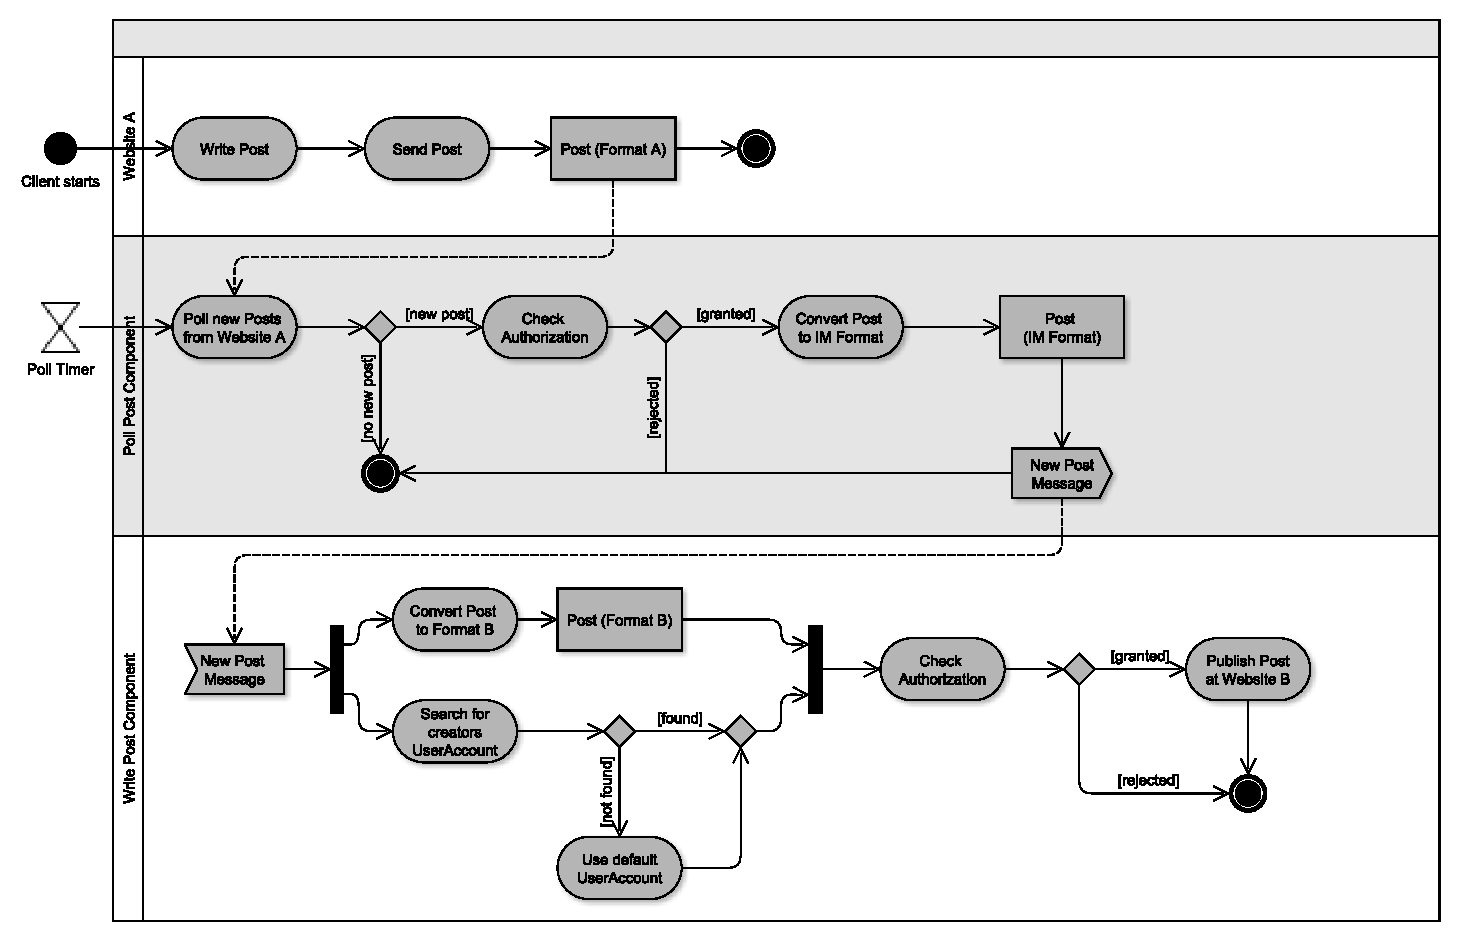
\includegraphics[
        width=\textwidth,
        keepaspectratio=true,
        clip=true,
        trim= 0 193 0 113
    ]{assets/images/activitydiagram_post_as_user_check_authorization.pdf}
    \caption{Daten lesen und in das Zwischenformat konvertieren}
% section beiträge_von_solzialen_netzwerk_a_lesen (end)
    \label{fig:lesen_von_beitrag_und_convertieren}
\end{figure}

\subsubsection{Wahl des Zwischenformats für die Datenkonvertierung} % (fold)
\label{ssub:wahl_des_zwischenformats_für_die_datenkonvertierung}

Ein passendes Zwischenformat wurde im Kapitel \enquote{\ref{cha:grundlagen}} mit SIOC beziehungsweise die Kombination aus SIOC und FOAF bereits vorgestellt. Damit ist es nicht nur möglich einzelne Beiträge plattformunabhängig zu speichern, sondern es kann auch die Struktur der Plattform als auch der Benutzer mit eingebunden werden. Auch können Maschinen aus den RDF-Daten einfach Wissen für neue, hilfreiche Informationen ableiten. Doch warum sollte man auf RDF und Ontologien setzen anstatt etwas eigenes zu Entwickeln wie auf Basis des weitverbreiteten und vielseitigen XML Formats?

Hier gibt es mehrere Vorteile, warum man RDF einer mit XML-Schema definierten XML-Datei vorziehen sollte. XML hat das Problem, dass die selbe Aussage auf verschiedene Art repräsentiert werden kann. Listing \ref{lst:xml_vs_rdf_multiple_rep} zeigt ein Beispiel für die Repräsentation der Aussage \enquote{Max Hiwi ist der Autor des Beitrags mit der ID 42} in XML.

\begin{lstlisting}[
    language=XML,
    caption={XML: Unterschiedliche Syntax, gleiche Semantik }\label{lst:xml_vs_rdf_multiple_rep},
    captionpos=t]
    <post>
        <id>42</id>
        <author>Max Hiwi</author>
    </post>

    <post id="42">
        <author>Max Hiwi</author>
    </post>

    <post id="42" author="Max Hiwi" />
\end{lstlisting}

Alle drei XML-Elemente beschreiben die selbe Aussage, aber auf unterschiedliche Art und Weise. Für einen Menschen haben diese drei Schreibweisen die selbe Aussage, für eine Maschine ist dies aber nicht mehr ganz so offensichtlich. Auch kann nicht die Bedeutung der einzelnen Element und Tags von Maschinen erfasst werde. Dies muss der Programmierer erledigen.Zusätzlich erschweren diese Unterschiedlichen Strukturen das ausführen von Abfragen auf diesen Daten, da ein Mapping zwischen einer logischen Abfrage und den Daten nicht eindeutig erfolgen kann (vgl. \cite[s.\,41]{Schroder2003a}).

% subsubsection wahl_des_zwischenformats_für_die_datenkonvertierung (end)

% subsection datenkonvertierung (end)

\subsection{Datenaustausch} % (fold)
\label{sub:datenaustausch}

Da das Eintreffen neuer Beitrage nicht vorhersagbar ist, ist es angebracht beim Synchronisieren das Lesen und Schreiben zeitlich zu entkoppeln. Eine der weit verbreitetsten Techniken dazu ist das Versenden von Nachrichten über einen Nachrichtenkanal den die schreibende Komponente nach neuen Beiträgen abhört. Diesen Kanal können mehrere Gleichzeitig abhören und stellen so eine gute Flexibilität sicher. 

\subsubsection{Wahl der Technik für den Datenaustausch} % (fold)
\label{ssub:wahl_der_technik_für_den_datenaustausch}

Dieses Verhalten lässt sich mit JMS und Camel gut implementieren. Doch welche von den zwei Technologien sollte man nutzen? JMS hat den Vorteil, dass das versenden von Nachrichten ohne großen Aufwand möglich ist, da die meiste Arbeit von der MOM übernommen wird und man selber nur die Nachrichten zusammenbauen und verarbeiten muss. Mit JMS können auch so hilfreiche Funktionen wie \enquote{Durable Subscriber} eingesetzt werden. Falls diese Funktion aktiviert ist und ein Client kurzzeitig keine Nachrichten empfangen kann (Zu ausgelastet oder die Verbindung ist abgebrochen), so speichert die MOM alle Nachrichten für diesen Client und schickt sie ihn erst, wenn er wieder verbunden ist. Da sich JMS nur um das Versenden und Empfangen kümmert, muss alles was darüber hinaus geht selbst implementiert oder nach zusätzlichen Bibliotheken gesucht werden.

Mit Camel ist es genauso wie mit JMS mögliche Nachrichten von einen System in ein anderes zu schicken. Mit Camal kann dafür im Gegensatz zu JMS die Route der Nachricht frei definiert und diverse Komponenten erweitert werden. So wäre es ohne Probleme möglich einen Filter für schlimme Worte in die Route einzubauen ohne etwas an den anderen Komponenten zu ändern. Camel hat aber das Problem, dass es ohne die richtigen Zusatzkomponenten Nachrichten nur innerhalb des selben Programms verschickten kann. Für das Verschicken über die Grenzen des Programms und des Systems hinaus müssen Komponenten in die Route eingebaut werden, die eine Netzwerkkommunikation anbieten. 

Die beste Wahl wäre eine Mischung aus JMS und Camel. So kann das entstehende System den Nachrichtenstrom durch auf einfache Art und Weise erweitern und umbiegen und durch JMS ist die Kommunikation über ein Netzwerk möglich und es stehen Funktionen wie der \enquote{Durable Subscriber} zur Verfügung.

% subsubsection wahl_der_technik_für_den_datenaustausch (end)

% subsection datenaustausch (end)

\subsection{Abschluss von Datenkonvertierung und -austausch} % (fold)
\label{sub:beiträge_in_eine_andere_webseite_schreiben}

Empfängt nun eine Komponente, die für das Schreiben zuständig ist, eine Nachricht von einen neuen Beitrags der Webseite A ist der Ablauf ähnlich wie beim Lesen nur in umgekehrter Reihenfolge (Siehe Abbildung \ref{fig:konvertieren_formatb_und_schreiben} links, oberer Ablauf). Der neue Beitrag wird vor dem Schreiben aus dem Zwischenformat in das Format B konvertiert. Da bei einer Synchronisation vom Vorteil wäre, wenn der synchronisierte Beitrag so aussehen würde, als hätte ihn der original Autor geschrieben. Hierzu muss das System Zugriff auf die Benutzerkonto haben und diese in einer Datenbank verwalten. Dort kann dann nach einen passenden Benutzerkonto des Autors gesucht und dieses dann zum Schreiben verwendet werden. Steht ein solches Benutzerkonto nicht zur Verfügung, ist das Ausweichen auf ein vorgegebenes Benutzerkonto hilfreich. Sind alle Voraussetzungen gegeben, kann der Beitrag mit dem ausgewählten Benutzerkonto auf die Webseite B geschrieben werden.

\begin{figure}[ht]
     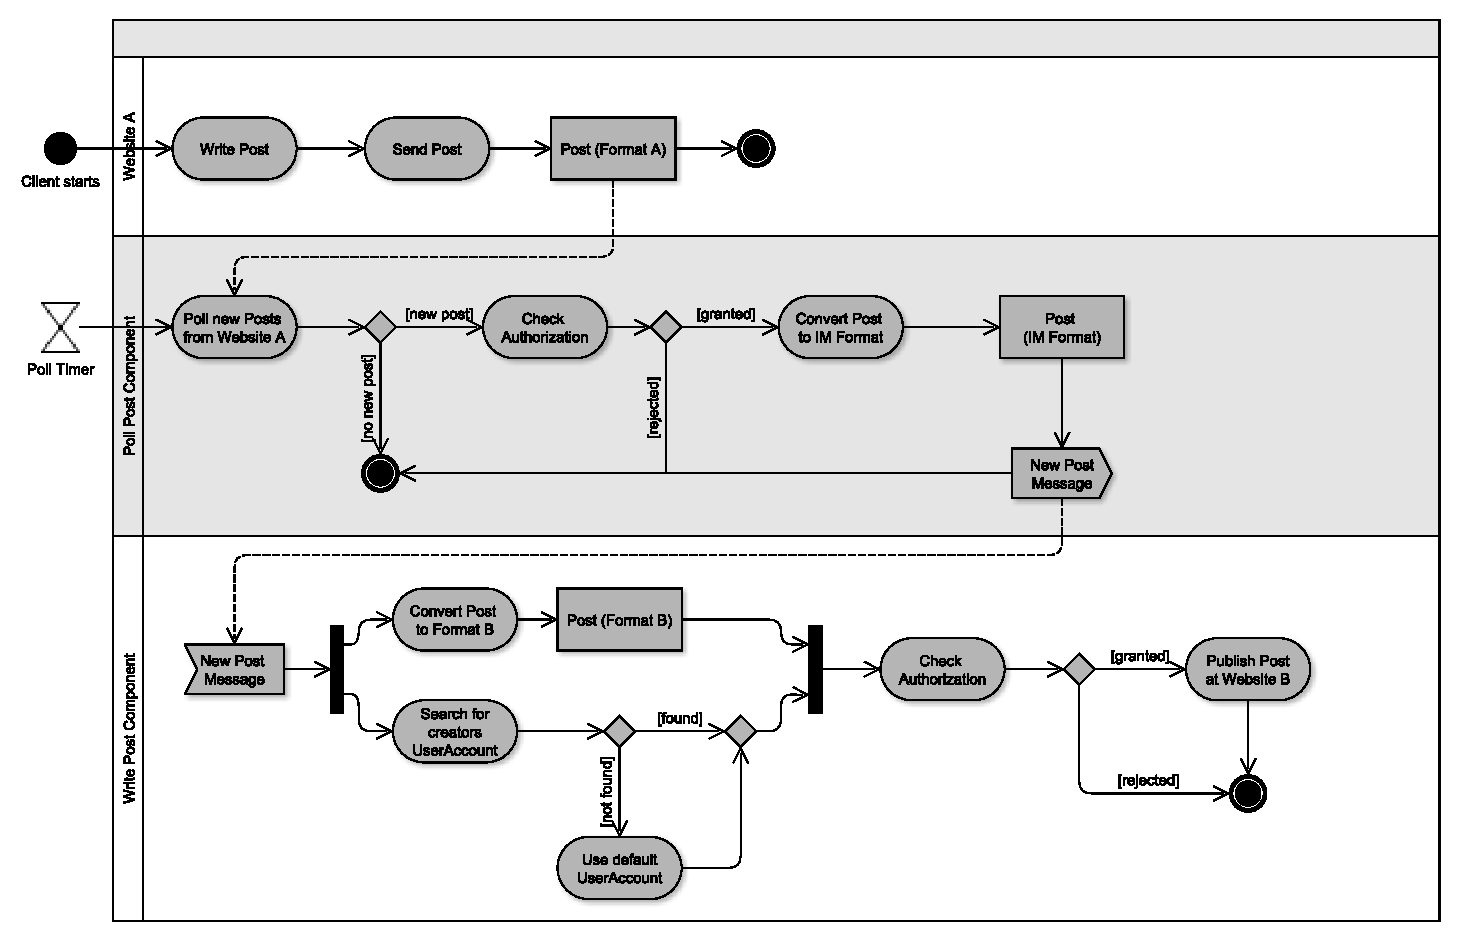
\includegraphics[
        width=\textwidth,
        keepaspectratio=true,
        clip=true,
        trim= 0 0 0 257
    ]{assets/images/activitydiagram_post_as_user_check_authorization.pdf}
    \caption{Konvertierten des Beitrags in das Format B und schreiben n das soziale Netzwerk B}
    \label{fig:konvertieren_formatb_und_schreiben}
\end{figure}

% subsection beiträge_in_eine_andere_webseite_schreiben (end)

\subsection{Privatsphäre} % (fold)
\label{sub:privatsphäre}

Wie in Abbildung \ref{fig:lesen_von_beitrag_und_convertieren} und \ref{fig:konvertieren_formatb_und_schreiben} des Ablaufdiagramms zu sehen ist, wird jeweils beim Lesen und Schreiben nach einer Autorisation gefragt. Bei der automatischen Sammlung von benutzergenerierten Inhalten stellt sich immer die Frage der Privatsphäre. Nicht jeder möchte, dass vielleicht sensible Informationen von ihnen weitergegeben werden oder ein Programm in seinen Namen Beiträge schreibt. Aus diesem Grund ist die Einführung eines Mechanismus sinnvoll mit dem ein Benutzer das Lesen seiner Beiträge und Schreiben in seinen Namen erlaubt, auf bestimmte Orte beschränkt oder verbietet (vgl. \cite[S.\,7]{Bojars2011}). 

% subsection privatsphäre (end)

\section{Identifizierung der Komponenten} % (fold)
\label{sec:identifizierung_der_komponenten}

Anhand dieser Schritte im Beispielszenario können sich eine Komponenten ablesen lasse, die das zu entwickelnde System enthalten muss. Gleichzeitig wurden einige Techniken ausgewählt auf die das System aufbauen kann, um nicht das komplette Rad neu erfinden zu müssen. 

\begin{itemize} 
    \item Eine Komponente muss eine einheitliche Schnittstelle definieren mit der die Daten eine beliebigen Webseite durch eine Öffentliche API gelesen und in das SIOC-Format konvertiert und von diesem wieder in eine andere Webseite geschrieben werden kann. 

    \item Die Beiträge im SIOC-Format sollen über Camel und JMS zwischen den Schnittstellen ausgetauscht werden können.

    \item Um stellvertretend für einen Benutzer schreiben zu können, muss es möglich sein nach dem Konto eines Benutzer zu einer bestimmten Webseite zu suchen suchen und für den Zugriff über die API zu nutzen.

    \item Um die Privatsphäre der Benutzer zu gewährleisten, ist ein Mechanismus zum Festlegen von Zugriffsrechen sinnvoll.
\end{itemize}   

% section identifizierung_der_komponenten (end)

% chapter analyse (end)